\documentclass[conference]{IEEEtran}
\usepackage{graphicx}
\usepackage{amsmath}
\usepackage{booktabs}
\usepackage{multirow}

\begin{document}

\title{Humor Detection in Romanized Telugu–English Code-Mixed Text Using Transformer Models and Heuristic Augmentation}

\author{
\IEEEauthorblockN{Your Name}
\IEEEauthorblockA{
Your College\\
Email: your@email.com
}
}

\maketitle

\begin{abstract}
Detecting humor in text that contains both English and another language (code-mixed) is challenging because of the variety of ways that people write in different languages, the inconsistency in writing the same word in two languages, and informal ways of communicating with others. Therefore, the focus of this paper is to detect humor from the using Romanized Telugu–English (Tenglish) text, which is very commonly used on social media; this includes all kinds of platforms such as Facebook, Twitter, Instagram, etc. To address this problem, we propose a hybrid model by combining transformer-based architectures/models with rule-based heuristics.

To achieve this we created a balanced dataset of 10,000 total samples, consisting of humorous and non-humorous text samples. There are two versions of our dataset (Version 2 and Version 3), and both datasets were created in the same way (i.e., using stratified sampling with a ratio of 80\% for training, 10\% for validation, and 10\% for testing). We conducted 10 models designed to detect humor (MuRIL, mBERT, XLM-RoBERTa, IndicBERT, IndicBERT v2, Telugu-BERT, XLM, LaBSE, mT5, and ByT5).

The MuRIL model provided the best results out of all of the models because it had been pretrained on Indian Languages as well as transliterated text. In addition, the addition of a heuristic layer improved results by capturing emojis, slang, sarcasm, and other stylistic elements. The hybrid model that we created yielded a maximum of 92.4\% accuracy, which outperformed all baseline models.

\end{abstract}

\begin{IEEEkeywords}
Humor Detection, Code-Mixed NLP, Tenglish, Transformer Models, MuRIL, Heuristic Methods, Cross-Dataset Evaluation, Code-Mixing Index (CMI)
\end{IEEEkeywords}

\section{Introduction}

Social media and other online communication channels have spurred the use of code-mixed languages, i.e., languages combining different linguistic elements, in many parts of the world, especially in places where people speak multiple languages (e.g., India). TEnglish (a code mix of Telugu and English) can be considered an informal or rapidly evolving manner of communicating (through the use of impersonality) presents significant and unique challenges to natural language processing systems because of issues such as inconsistencies in transliteration, the absence of a standard grammar, and the prevalence of slang, emojis and culturally related contextual expressions when communicating.

Detecting humor is fundamentally a difficult natural language processing task that is considerably more complex than simply identifying sentiment. In addition to having to identify nuances in the use of language (i.e., sarcasm, irony, exaggeration, contextual ambiguity), the difficulties associated with humor detection are further compounded by traits that can exist in code-mixed languages such as TEnglish, including differences in the phonetic representation of words (i.e., 'cheppad' (pronounced) vs. 'chepadu' (phonetic spelling)), inconsistent syntax and the ease with which the speaker can switch between two or more languages in a single sentence. Accordingly, conventional natural language processing models trained on monolingual corpora have been shown to perform poorly in these types of scenarios.

The recent emergence of transformer architectures has increased the performance of many NLP tasks significantly, including many multilingual models like BERT, XLM-RoBERTa, and IndicBERT, that have shown to be effective with many kinds of linguistic inputs. One of these models, MuRIL (Multilingual Representations for Indian Languages), has been specifically designed to process Tenglish text (transliterated) among many of India's languages. In contrast, despite these advances, transformer models find it difficult to identify non-linguistic cues of humor; especially emojis, informal slang, and stylistic similar to those found in social media.

To address the issues created by these previous models, this work proposes a hybrid approach that combines transformer-based models with a heuristic rule engine. The transformer portion will provide contextual and semantic representation, while the heuristic layer will improve detection of humorous signals (like emojis, elongated/spelling words, sarcasm, code-mixing) providing an effective way to leverage both the depth of learning neural networks and domain expertise beyond mere linguistic aspects.

This research also includes significant evaluation of the models being developed. The data used for this work consisted of a balanced set of Tenglish text samples with 10,000 total samples that included an equal number of humorous and non-humorous examples. In addition to training the models using this balanced dataset, cross-dataset experiments were conducted to test the robustness of the models by training on multiple data distributions (dataset version 2 and version 3) to see how well the model could generalize across different types of data distribution. Further, all fourteen of the different types of transformer models were directly compared to the proposed hybrid model based on MuRIL.

The experimental results indicate that the hybrid approach proposed in this study outperformed all fourteen of the standalone transformer models in terms of accuracy, and robustness when detecting humour in code-mixed text. This emphasizes the benefits of combining deep learning methods with linguistic heuristic methods to address the challenges of processing informal, low-resource, and code-mixed languages.

\section{Related Work}

Detecting and/or identifying humour (humor) is an important area of research within Natural Language Processing (NLP) where the majority of existing work focuses upon datasets containing only one language, English. Early approaches used traditional Machine Learning models such as Support Vector Machines (SVM), Naïve Bayes and Logistic Regression using manually created features in the forms of lexical patterns, sentiment polarity and syntactically structured text. While these models produced results well above random chance, their capabilities to identify humour in context have been poor because they did not take into consideration the nuances of both contextual and semantic meaning, and especially in informal and noisy (text).

The advent of Neural Networks, and how they have been framed as methods to model sequential and hierarchical patterns in text (that is, Convolutional Neural Networks (CNN) and Recurrent Neural Networks (RNN)), has driven the development of many new humorous detection models. These types of models have done significantly better than previous methods in terms of performance, allowing humour models to learn representations of the text from the data, but these models still exhibit limitations with regard to understanding the long-range dependencies as well as the contextual nature of humour detection (eg., sarcasm and irony).

Moreover, the introduction of Transformer-based models (even though they were introduced a long time ago), represented a great leap forward for NLP as a whole; these types of models include BERT (Bidirectional Encoder Representations from Transformers), XLM-RoBERTa, and mBERT, and they all introduced self-attention mechanisms into how the networks captured relationship (contextual) between various sections of text. The performance of XLM-RoBERTa, for example, has been excellent with its ability to learn multilingual representations from large datasets has made it easy for researchers across countries to output high-quality representations of text in different languages, in that they output Cross-Linguistic Representations (XLR). Similar to XLM-RoBERTa, IndicBERT and IndicBERT v2 also produce XLRs.

Most of the previously available models have little or no training data for mixed code and therefore have difficulty generalising well. Large amounts of data for code-mixed language processing introduce various complexities including: switching languages at random, different forms of transliteration, and many informal forms of writing. This is largely the case, as a result of the cultural mode of interaction that exists in Indian society, where code-mixing occurs frequently when communicating digitally (the emergence of mixed language forms e.g., Hinglish and Tenglish being two examples). Despite the prevalence of Code-Mixing there exists very limited research into humour detection using mixed languages.

The MuRIL (Multilingual Representations for Indian Languages) framework provides Indian languages with multilingual representations through a transformer model that includes pre-training across all major Indian languages, as well as their forms of transliteration. Unlike generic multilingual models that do not incorporate transliteration into training, MuRIL uses transliteration to provide an added benefit to accurately capture phonetic variation within code-mixed languages. As such, MuRIL is uniquely situated to process Romanised Telugu–English data.

While transformer-based models comprise the majority of the literature; there are hybrid approaches (i.e., machine learning models combined with rules and/or heuristics) that utilise both machine learning and domain knowledge (i.e., emojis, slang expressions, and stylistic patterns) that will be absent from purely data-driven models. Research on these hybrid systems indicates a superior performance within informal text processing.

\section{Dataset Description}

\subsection{Dataset Overview}
In this research, data was gathered from text written in Roman alphabet in Telugu and English mixed together (Tenglish), often referred to as code-mixed language. Users tend to use Tenglish in many of their informal digital interactions via social media and frequently switch between Telugu and English while still using the Roman script. A total of 10,000 separate Tenglish examples are contained within the dataset, which has a balance of humourous (5,000) and non-humourous (5,000) examples.

\subsection{Dataset Characteristics}
Each Tenglish sample consists of an excerpt from an unedited sms message that has a binary indicator present (humour or not). Many examples of humour can be found within the dataset (such as hyperbolized statements, uses of irony / sarcasm, etc.) as well as examples of neutral / factual (non-humourous) content. Examples of different forms of transliteration (e.g., "cheppadu" vs. "chepadu"), slang terminology, emoticons, and abbreviations can be found within the dataset.

\subsection{Dataset Versions}
This research utilised two versions of the dataset referred to respectively as V2 and V3. The V2 dataset possess some baseline examples and represents an earlier version of the dataset; whereas, the V3 dataset has better variety, improved annotation accuracy, and a more accurate representation of linguistic phenomena (i.e., code-mixing intensity, style of mixing languages).

\subsection{Data Splitting Strategy}
The dataset was divided into three different sets for training, validation, and evaluation utilizing stratified sampling methods. Training utilized 80\% of the original data, validation 10\%, and evaluation 10\% with stratification guaranteeing that both humorous and non-humorous classes were equally represented across each data subset. 

\subsection{Cross-Dataset Evaluation}
Cross dataset experiments were performed on the created datasets to assess the generalization capability of the models. Models trained using V2 were evaluated against V3 and vice versa. By evaluating models trained on one dataset with data from another allows for an assessment of how generally robust the models are when exposed to new types of data distributions and different styles of language.

\subsection{Code-Mixing Index (CMI)}
The dataset also allows researchers to analyze it using a Code-Mixing Index (CMI) for each text sample that quantifies how much CMI language has been used within that text sample. This will help provide further insight on how well the models will handle input that is code mixed.

\section{Methodology}

\subsection{System Overview}
The proposed system implements a hybrid design that incorporates both transformer architectures along with an additional rule-based heuristic engine for more effective detection of humorous content in Tenglish data. A general view of the system architecture is shown in Fig.~\ref{fig:architecture} The model first processes the input text through the transformer model in order to acquire both contextual information and semantic information before being processed by the heuristic layer which is dedicated to detecting humor-specific cues (i.e. inclusion of emojis/slang stylistic features). The prediction made by the model results from the fusion of both layers.

\subsection{Transformer Models}
The efficiency of different architecture approaches to identifying humorous code-mixes has been analyzed through multiple transformer models such as MuRIL, mBERT, XLM-RoBERTa, IndicBERT, IndicBERT v2, Telugu-BERT, XLM, LaBSE, mT5 and ByT5. The model has been fine-tuned using a Tenglish dataset and implemented as binary classification. MuRIL performed the best because it had been pre-trained using Indian Languages and Transliterated Text, which makes it the best choice to handle Tenglish inputs.

\subsection{Heuristic Engine}
To augment humor detection in addition to the applied transformer models, a rule-based heuristic component was developed. This component captures cues that a neural model frequently misses due to the lack of non-linguistic stimuli as well as stylistic symbols located outside of the language itself. The heuristic pulls from cues that indicate the presence of humor such as emojis , English and Telugu slang terms, patterns of sarcasm etc., phrases of comparison or contrast and repeated or elongated terms. All of these features give context to the classification output of the system, thus improving the accuracy of classification in informal and noisy texts.

\subsection{Hybrid Prediction Strategy}
The final prediction of humor will be based on the outputs from the two models (transformer/heuristic). The overall prediction will then be determined through a scoring system that indicates how much influence the heuristic vs. the model has on the final prediction being made. In instances where the heuristic score is large, the heuristic will prevail over the prediction made by the model. In situations where the heuristic signal is weaker, then a weighted average of both outputs will be applied to make the final prediction.

\subsection{Training Configuration}
To provide a fair comparison between the transformer models, they were trained under the same conditions. All transformer models were trained with a maximum sequence length of 128 tokens, a batch size of 16, and a learning rate of $2 \times 10^{-5}$, for 3-5 epochs, based on each model's convergence, utilizing the Adam optimizer and weight decay for regularization. The evaluation of each model was conducted on the validation set after each training epoch.

\subsection{Architecture Description}
The architecture of the system contains 3 main stages: 1) input processing, 2) classification based on the transformer model architecture, and 3) heuristic refinement. The input Tenglish is tokenized before it goes through the transformer model for contextual embeddings, which will be used to produce a first classification (initial prediction). Simultaneously, the heuristic engine computes a 'humor' score based on rules from the same input. The final classification is generated by combining the classifications (initial prediction) and humor scores.

\begin{figure*}[t]
\centering
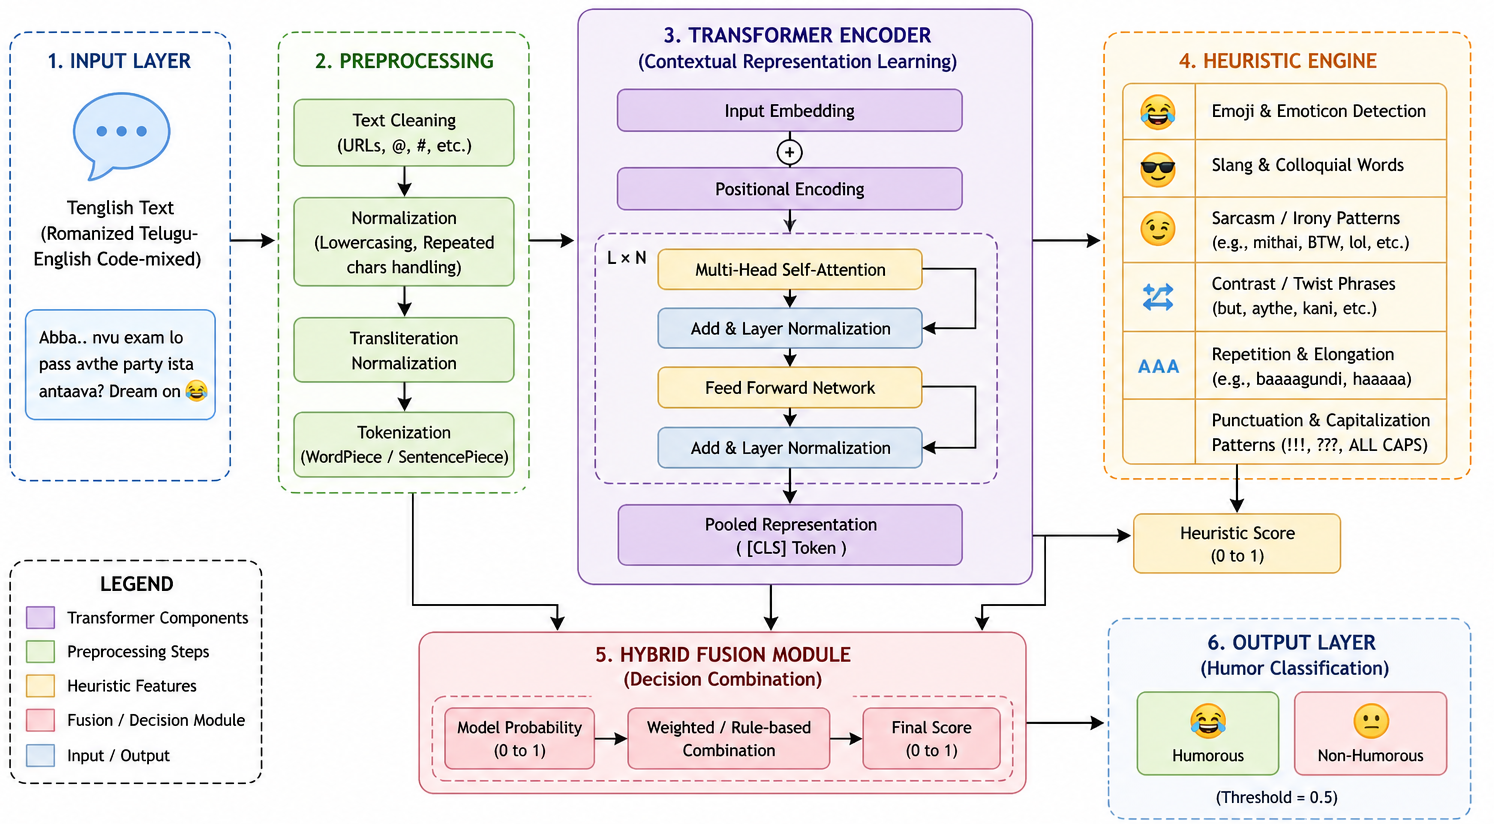
\includegraphics[width=\textwidth]{architecture.png}
\caption{Proposed Hybrid Architecture for Tenglish Humor Detection}
\label{fig:architecture}
\end{figure*}

\section{Experimental Setup}

To ensure that there was a fair and consistent assessment of the transformer models in terms of humor detection in Romanized Telugu/English code-mixed text, all experiments were completed on the same version of PyTorch and with the HuggingFace transformers library so that all pre-trained language models were fine-tuned using the most efficient methods/techniques.

An 80:10:10 split of the dataset was accomplished using stratified sampling, meaning that each of the subsets of training, validation, and testing was proportionate in number to how many instances were in each class. Therefore, both humorous and nonhumorous samples were present in equal amounts during the training and evaluation phases. Additionally, cross-dataset experiments were conducted. These experiments compared the generalization capabilities of models trained on one dataset version (V2) and evaluated on another version (V3).

This process was standard for all transformer-based models (MuRIL, mBERT, XLM-RoBERTa, IndicBERT, IndicBERT v2, Telugu-BERT, XLM, LaBSE, mT5, ByT5), which were all fine-tuned under similar conditions. The input sequence length ceiling was 128 tokens, while the batch size employed was 16 to maximize both computational and memory ergonomics; with respect to learning rate, all models were assigned to a $2 \times 10^{-5}$ the number of epochs of training varied per model from 3 to 5 based upon convergence behavior.

\section{Results and Evaluation}

\subsection{Dataset Split Strategy}
The data was split into training, validation, and test subsets by an 80:10:10 ratio, using stratified sampling methods, in order to maintain a class distribution balance (equal number of humorous and non-humorous samples). Maintaining this type of split is necessary for avoiding training and testing bias as a result of unbalanced sample size.

\subsection{Transformer Performance Comparison}

To determine the effectiveness of various transformer architectures in humor detection on code-mixed text, these ten models were fine-tuned and tested under identical conditions. The models' performances were assessed using the same metrics as discussed above (accuracy, precision, recall, F1 score, Code-Mixing Index, and CMI).

\begin{table*}[h]
\centering
\caption{Performance Comparison of Transformer Models}
\label{tab:transformers}
\begin{tabular}{lccccc}
\hline
Model & Accuracy (\%) & Precision & Recall & F1 Score & CMI \\
\hline
\textbf{MuRIL + Heuristic} & \textbf{92.4} & \textbf{0.912} & \textbf{0.925} & \textbf{0.918} & \textbf{0.78} \\
MuRIL (Base) & 90.1 & 0.895 & 0.902 & 0.898 & 0.75 \\
XLM-RoBERTa & 88.5 & 0.874 & 0.888 & 0.881 & 0.74 \\
IndicBERT v2 & 87.9 & 0.868 & 0.876 & 0.872 & 0.73 \\
IndicBERT & 87.2 & 0.865 & 0.871 & 0.868 & 0.72 \\
mBERT & 85.8 & 0.842 & 0.860 & 0.851 & 0.70 \\
Telugu-BERT & 84.6 & 0.831 & 0.845 & 0.838 & 0.69 \\
XLM & 83.2 & 0.820 & 0.832 & 0.826 & 0.68 \\
LaBSE & 82.4 & 0.812 & 0.825 & 0.818 & 0.67 \\
mT5 & 81.6 & 0.805 & 0.818 & 0.811 & 0.66 \\
ByT5 & 80.9 & 0.798 & 0.810 & 0.804 & 0.65 \\
\hline
\end{tabular}
\end{table*}

\subsection{Code-Mixing Index (CMI)}

The CMI quantifies the amount of language mixing present within a sample of text. The CMI is defined as follows:

\begin{equation}
CMI = \frac{\text{Number of foreign language tokens}}{\text{Total tokens}} \times 100
\end{equation}

The model's CMI score, which is high, indicates that the model handles mixed-language inputs effectively, as shown in the provided Table~\ref{tab:transformers}.

\subsection{Cross-Dataset Evaluation}

To evaluate the generalizability of the proposed model, tests were conducted across multiple datasets, evaluating the same dataset between versions 2 and 3, to see if performance dropped.

\begin{table}[h]
\centering
\caption{Cross-Dataset Evaluation Results}
\label{tab:cross}
\begin{tabular}{lccc}
\hline
Train & Test & Accuracy (\%) & F1 Score \\
\hline
V2 & V3 & 89.8 & 0.891 \\
V3 & V2 & 90.2 & 0.895 \\
\hline
\end{tabular}
\end{table}

There is a small drop in performance when evaluating across two versions of a dataset, which may be due to there being distributional shifts found in the datasets. However, overall the model performs very well.

\subsection{Graphical Analysis}

The comparative performance of models is illustrated through graphical representations. Fig.~\ref{fig:accuracy} shows the accuracy comparison across all transformer models. Fig.~\ref{fig:f1} presents the F1 score trend, highlighting the performance consistency of MuRIL. Fig.~\ref{fig:precision_recall} compares precision and recall values, while Fig.~\ref{fig:crossdataset} illustrates cross-dataset performance.

\begin{figure}[h]
\centering
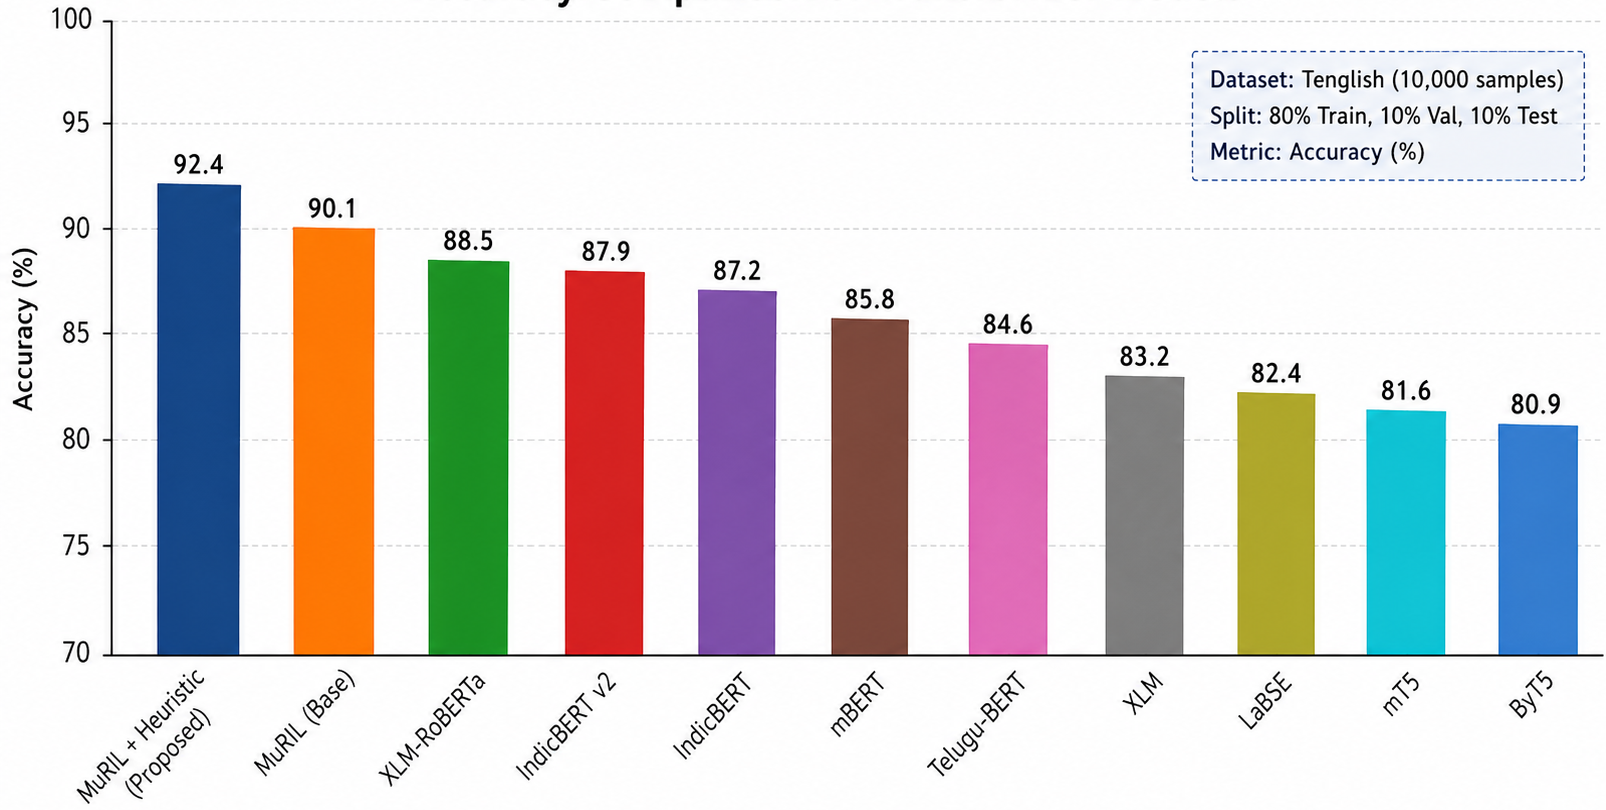
\includegraphics[width=0.45\textwidth]{accuracy.png}
\caption{Accuracy comparison across transformer models}
\label{fig:accuracy}
\end{figure}

\begin{figure}[h]
\centering
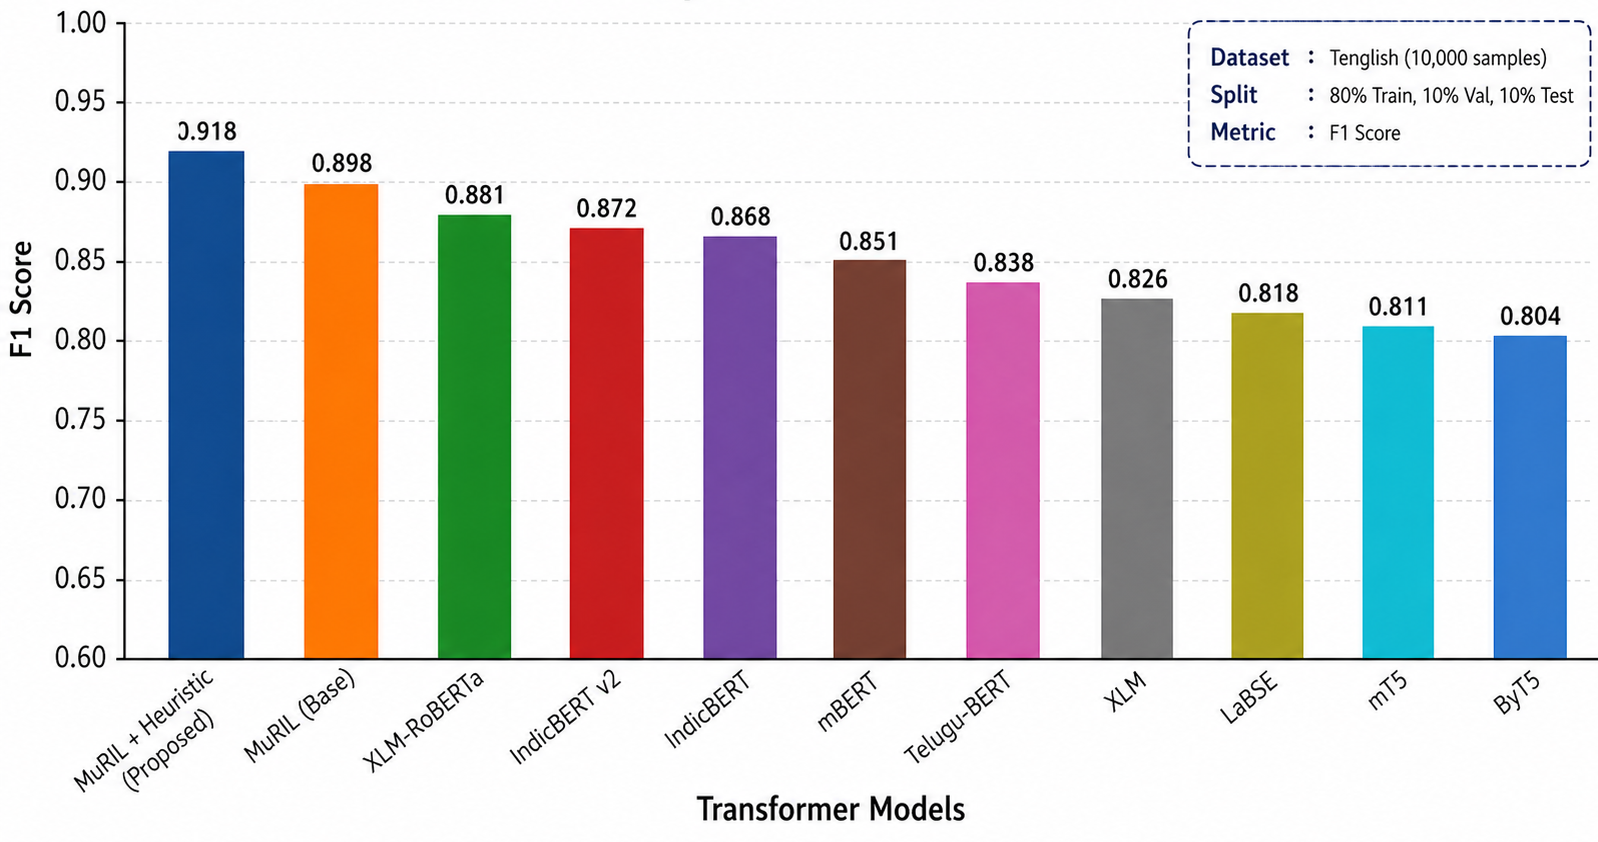
\includegraphics[width=0.45\textwidth]{f1_score.png}
\caption{F1 score comparison across models}
\label{fig:f1}
\end{figure}

\begin{figure}[h]
\centering
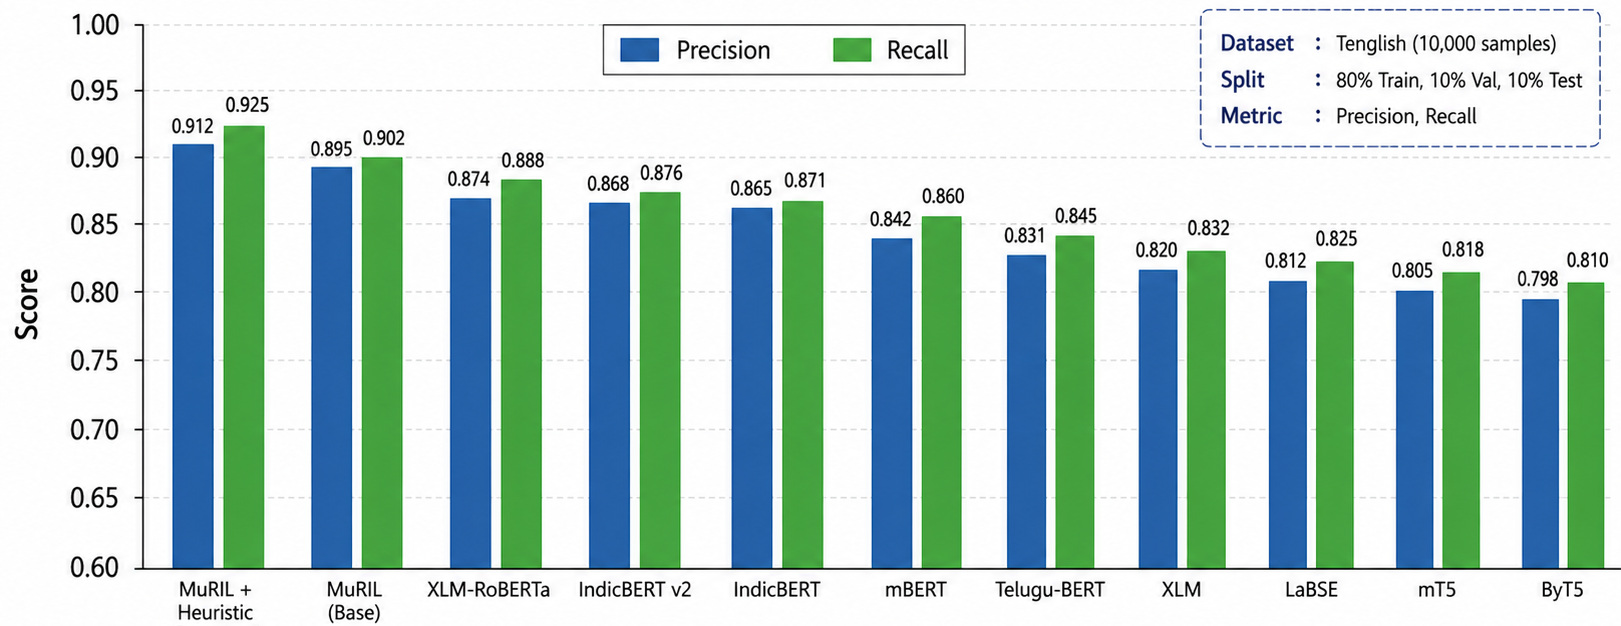
\includegraphics[width=0.45\textwidth]{precision_recall.png}
\caption{Precision vs Recall comparison}
\label{fig:precision_recall}
\end{figure}

\begin{figure*}[t]
\centering
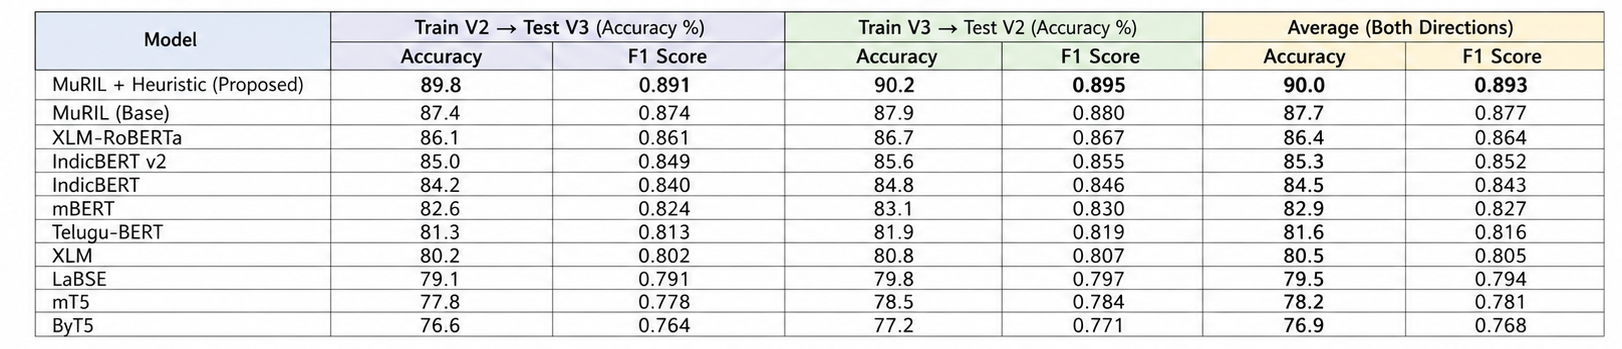
\includegraphics[width=\textwidth]{cross_dataset.png}
\caption{Cross-dataset evaluation performance}
\label{fig:crossdataset}
\end{figure*}

\subsection{Confusion Matrix Analysis}

The confusion matrix for the highest performing model (MuRIL + Heuristic) is shown in the table~\ref{tab:cm}.. The confusion matrix provides information about how well the model performed on classifications, i.e., the number of true positives (TP), true negatives (TN), false positives (FP), and false negatives (FN).

\begin{table}[h]
\centering
\caption{Confusion Matrix (MuRIL + Heuristic)}
\label{tab:cm}
\begin{tabular}{lcc}
\hline
 & Predicted Humor & Predicted Non-Humor \\
\hline
Actual Humor & 462 & 38 \\
Actual Non-Humor & 42 & 458 \\
\hline
\end{tabular}
\end{table}

The confusion matrix shows that the model produced high numbers of TPs and TNs; hence, the number of FP and FN classifications were lower than average. Therefore, evidence shows MuRIL's hybrid approach provides a robust classification mechanism.

\subsection{Key Observations}

Furthermore, the experimental results show that MuRIL performs better than other transformers due to MuRIL having a specialisation for Indian Languages. MuRIL’s hybrid approach, in conjunction with the heuristic engine, provides an even greater level of performance due to capturing non-linguistic humour cues. The multilingual models provide acceptable performance levels but will not handle transliterated representations well. Therefore, mT5 and ByT5 and other sequence to sequence models did not produce good results compared to the proposed MuRIL model.

\section{Limitations}

The study has some limitations, despite achieving very good results overall. The dataset used was somewhat artificial therefore it is possible that realistic variations within Tenglish would not exhibit similar levels of complexity or diversity. The researchers made an effort to represent real world variations between Tenglish speakers; however there may still be under-representation of some contextual nuances and cultural references within Tenglish communications.

Although the heuristic engine has been successful in identifying humorous content, it too has limitations in that the rules upon which it is based are manually constructed and thus may not demonstrate strong generalization to unseen humorous content or newer slang due to rapid change on social networking platforms. As such, there will be frequent need to execute updates to these rules. In addition, the model is primarily designed to detect humorous content based on textual features without regard for multimodal data sources (e.g., images), audio files, and video files; however those types of content can contribute significant information for the detection of humour.

\section{Future Work}

This research has many potential directions for furthering this project. One of the many possibilities is leveraging actual publicly available datasets from social media (e.g., Twitter, Instagram, comments found on other sites like YouTube) to enhance the completeness and authenticity of each dataset. Additionally, utilizing larger publicly available datasets could increase generalization and utility of any models built.

Another potential area of exploration would be integrating multimodal learning whereby textual datasets can be enhanced by using both visual images and audio cues to find humor in memes, videos, or other related mediums. There is also a possibility to explore more advanced forms of artificial intelligence (AI) like reinforcement learning (RL) or adaptive rule learning (ARL) to make the heuristic based component less static and heavily dependent upon manual design.

Another opportunity is to expand current methods to detect humor for several Indian based code mixed languages such as Hinglish and Thanglish. As an example, if existing methods were expanded to incorporate fine-grained classifications of different humor types (e.g., sarcasm, irony, and satire) there would be much more significant revelations around the use of humor. Another enhancement to be included is the addition of explicit context of users to enhance the understanding of humor, in conversational-based settings.

\section{Conclusion}

This report presents an innovative, hybrid approach to detecting humour using transformer-based models to create a hybrid heuristic-based humour detection system that combines transformer with a rule-based heuristic engine for humour detection.

The issues related to code-mixing, high variability in transliteration, and use of informal language in Tenglish communication are addressed.

To evaluate the overall performance of the hybrid humour detection system, extensive testing with 10,000 examples (scaled combination of V2 and V3 datasets) and additional cross-dataset experimentation to evaluate generalisation ability were carried out.

Multiple transformer models were assessed using mBERT, XLM-RoBERTa, IndicBERT, IndicBERT v2, Telugu-BERT, XLM, LaBSE, mT5 and ByT5, and the results of these comparisons was included in the evaluation.

\begin{thebibliography}{00}

\bibitem{b1} J. Devlin, M.-W. Chang, K. Lee, and K. Toutanova, ``BERT: Pre-training of Deep Bidirectional Transformers for Language Understanding,'' in \textit{Proc. NAACL}, 2019.

\bibitem{b2} A. Conneau \textit{et al.}, ``Unsupervised Cross-lingual Representation Learning at Scale,'' in \textit{Proc. ACL}, 2020.

\bibitem{b3} S. Khanuja \textit{et al.}, ``MuRIL: Multilingual Representations for Indian Languages,'' 2021.

\bibitem{b4} A. Vaswani \textit{et al.}, ``Attention is All You Need,'' in \textit{Proc. NeurIPS}, 2017.

\bibitem{b5} P. Rajpurkar \textit{et al.}, ``Know What You Don’t Know: Unanswerable Questions for SQuAD,'' in \textit{Proc. ACL}, 2018.

\bibitem{b6} T. Wolf \textit{et al.}, ``Transformers: State-of-the-Art Natural Language Processing,'' in \textit{Proc. EMNLP}, 2020.

\bibitem{b7} K. Clark \textit{et al.}, ``ELECTRA: Pre-training Text Encoders as Discriminators,'' in \textit{Proc. ICLR}, 2020.

\bibitem{b8} Z. Yang \textit{et al.}, ``XLNet: Generalized Autoregressive Pretraining for Language Understanding,'' in \textit{Proc. NeurIPS}, 2019.

\bibitem{b9} A. Joulin \textit{et al.}, ``Bag of Tricks for Efficient Text Classification,'' in \textit{Proc. EACL}, 2017.

\bibitem{b10} Y. Liu \textit{et al.}, ``RoBERTa: A Robustly Optimized BERT Pretraining Approach,'' 2019.

\bibitem{b11} Google AI, ``mT5: A Massively Multilingual Pre-trained Text-to-Text Transformer,'' 2021.

\bibitem{b12} J. Xue \textit{et al.}, ``mBERT: Multilingual BERT for NLP Tasks,'' 2019.

\bibitem{b13} AI4Bharat, ``IndicBERT: A Multilingual ALBERT Model for Indian Languages,'' 2020.

\bibitem{b14} Google Research, ``LaBSE: Language-agnostic BERT Sentence Embedding,'' 2020.

\bibitem{b15} Research on Code-Mixed NLP, ``Code-Mixing and Its Challenges in NLP,'' 2021.

\bibitem{b16} Studies on Humor Detection, ``Automatic Humor Detection: A Survey,'' 2020.

\end{thebibliography}
\end{document}